\renewcommand{\theequation}{\theenumi}
\begin{enumerate}[label=\arabic*.,ref=\thesubsection.\theenumi]
\item Find the equation of a circle which passes through the points $\myvec{2\\-1}$, $\myvec{1\\-2}$ and cuts orthogonally the circle
\begin{align}
\vec{x}^T\vec{x}+\myvec{-2 & 3}\vec{x}-5 = 0
\end{align}
\numberwithin{equation}{enumi}
Find the equation of a circle which cuts orthogonally the three circles
\begin{align}
    \vec{x}^T\vec{x} + \myvec{4&-5}\vec{x} + 6 = 0\label{4/4/2/circle1}\\
    \vec{x}^T\vec{x} + \myvec{5&-6}\vec{x} + 7 = 0\label{4/4/2/circle2}\\
    \vec{x}^T\vec{x} - \myvec{1&1}\vec{x} - 1 = 0\label{4/4/2/circle3}
\end{align}
\solution
\begin{lemma}
Tangent to a circle : Consider a circle 
\begin{align}
    \vec{x}^\top\vec{x} + 2\vec{c}^\top\vec{x} + f = 0 
\end{align}
Given a point $\vec{q}$ on the circle, the tangent at that point is given as,
\begin{align}
    \brak{\vec{q}+\vec{c}}^\top\vec{x} + \vec{c}^\top\vec{q} + f = 0 
\end{align}
\end{lemma}
\begin{lemma}
Orthogonality of circles : Two circles are said to be orthogonal if  the tangents at their points of intersection are perpendicular to each other.\\ That implies, tangents to one circle at the points of contact are normals to the other circle. 
Given two circles,
\begin{align}
    \vec{x}^\top\vec{x} + 2\vec{c_1}^\top\vec{x} + f_1 = 0 \label{4/4/2/eq1}\\
    \vec{x}^\top\vec{x} + 2\vec{c_2}^\top\vec{x} + f_2 = 0 \label{4/4/2/eq2}
\end{align}
They are orthogonal if
\begin{align}
    2\vec{c_1}^\top\vec{c_2} = f_1 + f_2 \label{4/4/2/condition}
\end{align}
\end{lemma}
\begin{proof}
Let the two circles \eqref{4/4/2/eq1} and \eqref{4/4/2/eq2} meet at a point $\vec{q}$ i.e $\vec{q}$ satisfies the equation of the circles
\begin{align}
    \vec{q}^\top\vec{q} + 2\vec{c_1}^\top\vec{q} + f_1 = 0 \label{4/4/2/2.0.4}\\
    \vec{q}^\top\vec{q} + 2\vec{c_2}^\top\vec{q} + f_2 = 0 \label{4/4/2/2.0.5}
\end{align}
Eliminating quadratic term,
\begin{align}
    2\brak{\vec{c_1}^T - \vec{c_2}^T}\vec{q} + f_1 - f_2 = 0 \label{4/4/2/2.0.6}
\end{align}
Given the point of contact $\vec{q}$, the equation of tangent to circle \eqref{4/4/2/eq1} is
\begin{align}
    \brak{\vec{q}+\vec{c_1}}^\top\vec{x} + \vec{c_1}^\top\vec{q} + f_1 = 0 
\end{align}
As it is a normal to the second circle \eqref{4/4/2/eq2}, it passes through the center of it
\begin{align}
    \brak{\vec{q}+\vec{c_1}}^\top\brak{\vec{-c_2}} + \vec{c_1}^\top\vec{q} + f_1 = 0 \\
    \implies \brak{\vec{c_1}^T - \vec{c_2}^T}\vec{q} + f_1 - \vec{c_1}^T\vec{c_2} = 0 \\
    \implies \brak{\vec{c_1}^T - \vec{c_2}^T}\vec{q} = \vec{c_1}^T\vec{c_2} - f_1
    \label{4/4/2/2.0.10}
\end{align}
Substituting \eqref{4/4/2/2.0.10} in \eqref{4/4/2/2.0.6},
\begin{align}
    2\brak{\vec{c_1}^T\vec{c_2} - f_1}  + f_1 - f2 = 0 \\
    \implies 2\vec{c_1}^\top\vec{c_2} = f_1 + f_2 
\end{align}
\end{proof}
\begin{lemma}
For given three circles,
\begin{align}
    \vec{x}^\top\vec{x} + 2\vec{c_1}^\top\vec{x} + f_1 = 0 \label{4/4/2/S1=0}\\
    \vec{x}^\top\vec{x} + 2\vec{c_2}^\top\vec{x} + f_2 = 0 \label{4/4/2/S2=0}\\
    \vec{x}^\top\vec{x} + 2\vec{c_3}^\top\vec{x} + f_3 = 0 \label{4/4/2/S3=0}
\end{align}
The equation of a circle $S$ which cuts these circles orthogonally is given by,
\begin{align}
    \vec{x}^\top\vec{x} + 2\vec{c}^\top\vec{x} + f = 0 \label{4/4/2/S=0}
\end{align}
Where 
\begin{align}
    \myvec{\vec{c}\\f} = \myvec{2\vec{c_1}^\top&-1\\2\vec{c_2}^\top&-1\\2\vec{c_3}^\top&-1}^{-1}\myvec{f_1\\f_2\\f_3}
\end{align}
\end{lemma}\label{4/4/2/lemma2}
\begin{proof}
Since $S$ is orthogonal to \eqref{4/4/2/S1=0}, \eqref{4/4/2/S2=0} and \eqref{4/4/2/S3=0} we have,
\begin{align}
    2\vec{c_1}^\top\vec{c} - f &= f_1\\
    2\vec{c_2}^\top\vec{c} - f &=  f_2\\
    2\vec{c_3}^\top\vec{c} - f &= f_3\\
    \implies \myvec{2\vec{c_1}^\top&-1\\2\vec{c_2}^\top&-1\\2\vec{c_3}^\top&-1}\myvec{\vec{c}\\f} &= \myvec{f_1\\f_2\\f_3}\\
\end{align}
\end{proof}
Let the required equation of the circle be
\begin{align}
    \vec{x}^\top\vec{x} + 2\vec{c}^\top\vec{x} + f = 0
\end{align}
It is orthogonal to the circles \eqref{4/4/2/circle1}, \eqref{4/4/2/circle2} and \eqref{4/4/2/circle3}
\begin{align}
    \implies \myvec{4&-5&-1\\5&-6&-1\\-1&-1&-1}\myvec{\vec{c}\\f} = \myvec{6\\7\\-1}
\end{align}
Therefore the augmented matrix can be transformed as,
 \begin{align}
		\myvec{4 & -5 & -1 & 6\\
		       5 & -6 & -1 & 7\\
		       -1 & -1 & -1 &-1}\\
		\xleftrightarrow[]{R_1\leftrightarrow-R_3 }
		\myvec{1 & 1 & 1 & 1\\
		       5 & -6 & -1 & 7\\
		       4 & -5 & -1 & 6}\\
		\xleftrightarrow[R_2 \leftarrow R_2-5R_1, R_2 \leftarrow -\frac{R_2}{11}]{R_3 \leftarrow R_3-4R_1}
		\myvec{1 & 1 & 1 & 1\\
		       0 & 1 & \frac{6}{11} & \frac{-2}{11}\\
		       0 & -9 & -5 &2}\\
		\xleftrightarrow[R_1 \leftarrow R_1-R_2]{R_3 \leftarrow R_3+9R_2}
		\myvec{1 & 0 & \frac{5}{11} & \frac{13}{11}\\[0.2cm]
		       0 & 1 & \frac{6}{11} & \frac{-2}{11}\\[0.2cm]
		       0 & 0 & \frac{-1}{11} & \frac{4}{11}}\\
		\xleftrightarrow[R_1 \leftarrow R_1+5R_3, R_3 \leftarrow -11R_3]{R_2 \leftarrow R_2+6R_3}
		\myvec{1 & 0 & 0 & 3\\ 
		       0 & 1 & 0 & 2\\
		       0 & 0 & 1 &-4}\\
    \implies \vec{c} = \myvec{3\\2}, f = -4 		       
\end{align}

The required equation of circle,
\begin{align}
    S = \vec{x}^\top\vec{x} + \myvec{6&4}\vec{x} - 4 = 0
\end{align}
\begin{figure}[h!]
\centering
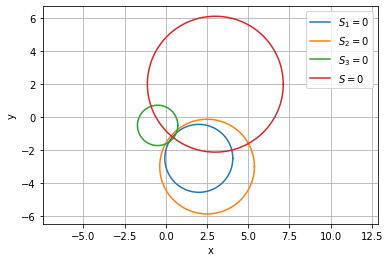
\includegraphics[width=\columnwidth]{solutions/4/4/2/figures/CirclesPlot.png}
\caption{Plot of circles}
\label{4/4/2/fig:circles plot}
\end{figure}


\item Find the equation of a circle which cuts orthogonally the two circles
\begin{align}
\vec{x}^T\vec{x}-\myvec{2 & 2}\vec{x}+1 = 0
\\
\vec{x}^T\vec{x}+\myvec{-3 & 6}\vec{x}-2 = 0
\end{align}
and passes through the point $\myvec{-3\\2}$.
\item Write down the equations of the radical axes of the following pairs of circles:
\begin{enumerate}
\item
%
\begin{align}
\vec{x}^T\vec{x}-\myvec{4 & -5}\vec{x}-2 = 0
\\
\vec{x}^T\vec{x}-\myvec{5 & -6}\vec{x} = 0
\end{align}
%
\item
\begin{align}
%
\vec{x}^T\vec{x}+\myvec{3 & -2}\vec{x}+1 = 0
\\
\vec{x}^T\vec{x}-\myvec{3 & -5}\vec{x}+2 = 0
\end{align}
%
\item
\begin{align}
%
\vec{x}^T\vec{x}+2g\myvec{1 & 0}\vec{x}+c = 0
\\
\vec{x}^T\vec{x}+2f\myvec{0 & 1}\vec{x}+c = 0
\end{align}
%
\end{enumerate}
\solution

Given, two circles with equations,
\begin{align}
S=\vec{x}^{T}\vec{x}-\myvec{4 & -5}\vec{x}-2=&0\label{rams/4/4/4/a/eq:1}\\
S'=\vec{x}^{T}\vec{x}-\myvec{5 & -6}\vec{x}=&0\label{rams/4/4/4/a/eq:2}
\end{align}
We know, the radical axis for the pair of circles, $S=0, S'=0$ is given by $L=S-S'=0$.\\
Using \eqref{rams/4/4/4/a/eq:1}, \eqref{rams/4/4/4/a/eq:2}, the required equation is
\begin{align}
\brak{\vec{x}^{T}\vec{x}-\myvec{4 & -5}\vec{x}-2}-\brak{\vec{x}^{T}\vec{x}-\myvec{5 & -6}\vec{x}=0}=&0\\
\myvec{1 & -1}\vec{x}-2=&0
\end{align}
$\therefore L=\myvec{1 & -1}\vec{x}-2=0$ is the equation of the required radical axis.  See Fig.  \ref{rams/4/4/4/a/plot}
\begin{figure}[!h]
 \centering
 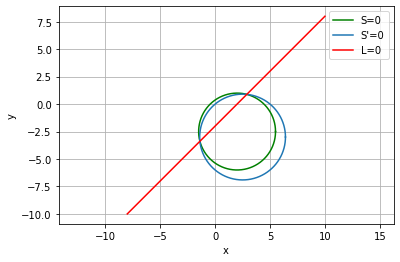
\includegraphics[width=\columnwidth]{solutions/4/4/4/a/figures/Assignment3.png}
 \caption{Pair of Circles and their radical axis}
 \label{rams/4/4/4/a/plot}
\end{figure}

\item Find the equation of a circle coaxal with
\begin{align}
\vec{x}^T\vec{x}-\myvec{2 & -3}\vec{x}-1 &= 0
\\
\vec{x}^T\vec{x}+\myvec{3 & -2}\vec{x}-1 &= 0
\end{align}
and passing through the point $\myvec{2\\1}$.
\item Find the coordinates of the point from which the tanges to the three circles
\begin{align}
\vec{x}^T\vec{x}-\myvec{4 & 4}\vec{x}+7 = 0
\\
\vec{x}^T\vec{x}+\myvec{4 & 0}\vec{x}+3 = 0
\\
\vec{x}^T\vec{x}+\myvec{0 & 2}\vec{x} = 0
\end{align}
are of equal length.
\item Find the limiting points of the circles
\begin{align}
\vec{x}^T\vec{x}+\myvec{0 & 2}\vec{x}-4 &= 0
\\
\vec{x}^T\vec{x}+\myvec{2 & 2}\vec{x}-10 &= 0
\end{align}
\item Prove that if a point moves so that the tangent from it to the circle
\begin{align}
\vec{x}^T\vec{x}+\myvec{4 & -5}\vec{x}+6 = 0
\end{align}
is double the length of the tangent to the circle
\begin{align}
\norm{\vec{x}} = 2,
\end{align}
its locus is the circle
\begin{align}
3\vec{x}^T\vec{x}-\myvec{4 & -5}\vec{x}-22 = 0
\end{align}
\item Prove that the locus of a point such that the lengths of the tangents from it to two given circles are in a constant ratio is a circle
coaxal with the given circles.
\item Find the equations of the two circles coaxal with
\begin{align}
\vec{x}^T\vec{x}-\myvec{8 & -10}\vec{x}+2 = 0
\\
\vec{x}^T\vec{x}-\myvec{3 & -5}\vec{x}-1 = 0
\end{align}
that touch the line
\begin{align}
\myvec{2 & 1}\vec{x}-3 = 0
\end{align}
\item Find the centre and radius of the circle which cuts orthogonally the three circles
\begin{align}
\vec{x}^T\vec{x}-\myvec{6 & 4}\vec{x}+12 = 0
\\
\vec{x}^T\vec{x}+2\myvec{1 & 1}\vec{x}+1 = 0
\\
\vec{x}^T\vec{x}+\myvec{4 & -2}\vec{x}+4 = 0
\end{align}
\item The line 
\begin{align}
\myvec{1 & 3}\vec{x}+2 = 0
\end{align}
is the radical axis of a family of coaxal circles of which one circle is
\begin{align}
\vec{x}^T\vec{x}+\myvec{2 & 5}\vec{x}-1 = 0.
\end{align}
Find the equation of the member of the family that passes through the point $\myvec{-3\\1}$.
\end{enumerate}
